% !TEX root = ../main.tex

% ---------------------------------------------------------------
% Software Implamentation of metodology
% ---------------------------------------------------------------
\chapter[Risultati Sperimentali]{Risultati Sperimentali}\label{chap6:result}
In questo capitolo, verranno descritti i risultati sperimentali ottenuti per ogni fase descritta nel capitolo precedente.

\section{Dataset}
L'approccio che andiamo a proporre è stato testato sul dataset DAPHNET\footnote{www.wearable.ethz.ch/resources/Dataset}, il quale contiene dati collezionati da 10 pazienti parkinsoniani, dei quali 8 presentano contesti di FoG, mentre 2 di loro non ne hanno. I dati sono stati registrati usando 3 accelerometri 3D, quindi a tre assi x,y,z, attaccati alla caviglia, al ginocchio e nella zona lombare del paziente, usando una frequenza di campionamento di 64 Hz.\\
I soggetti hanno completato sessioni da 20-30 minuti ciascuno, consistenti di 3 fasi di camminata:
\begin{enumerate}
	\item Camminata avanti ed indietro lungo una linea retta, con delle rotazioni di 180 gradi;
	\item Camminata casuale con una serie di fermate volontarie e rotazioni di 360 gradi;
	\item Camminata che simula attività di vita quotidiana, tra le quali entrare in stanze ed uscirne, camminare nella cucina, prendersi un bicchiere d'acqua e tornare al punto di partenza.
\end{enumerate}
Le prestazioni motorie variano molto tra i pazienti. Mentre alcuni soggetti hanno mantenuto una camminata regolare durante gli episodi di non FoG, altri hanno camminato molto lentamente ed in modo instabile. L'intero dataset contiene in totale 237 episodi di FoG; la durata di ognuno di essi è tra i 0.5s ed i 40.5s. Il 50\% degli episodi di FoG è durato meno di 5.4s ed il 93.2\% è più corto di 20s. Gli episodi di FoG sono stati identificati da fisioterapisti usando registrazioni video sincronizzate. L'inizio di un episodio di FoG è stato definito come il punto dove la sequenza normale di camminata è stata interrotta, mentre la fine del FoG è stata definita come il momento in cui tale sequenza riprende.

\section{Risultati sull'esistenza della classe preFOG}
La fase 1 si prefiggeva l'obiettivo di verificare che la classe preFOG potesse essere differenziata dalle altre due classi, ossia quella di noFOG e FOG. Per visualizzare se effettivamente esiste una distinzione tra le classi, tracciamo un grafico con le grandezze derivanti dalla procedura di LDA, in cui ogni punto viene colorato in base alla reale classe di appartenenza.\\
Le figure \ref{LDAS01} e \ref{LDAS02} fanno notare immediatamente come le feature utilizzate riescono a discriminare abbastanza tra le 3 classi, anche se c'è ancora una certa sovrapposizione tra i dati di classi diverse, almeno usando i dati di un solo paziente.\\
Ogni soggetto, però, ha dei pattern di camminata diversi, quindi posso avere dati molto differenti tra un paziente ed un altro. Abbiamo quindi verificato anche se, utilizzando i dati di tutti i pazienti, la discriminazione lineare riesce ancora a distinguere tra le varie classi.\\
La figura \ref{LDAALL} mostra che, usando i dati di tutti i pazienti assieme, una certa divisione rimane, anche se è molto meno netta rispetto a quella del singolo paziente. Questo comunque ci permette di dire che anche tra pazienti differenti, quindi con pattern di cammino diversi, i dati di preFOG sono abbastanza divisi da quelli di noFOG o FoG, quindi un approccio concentrato su questa nuova classe sembra sensato.

\begin{figure}[]
	\centering
	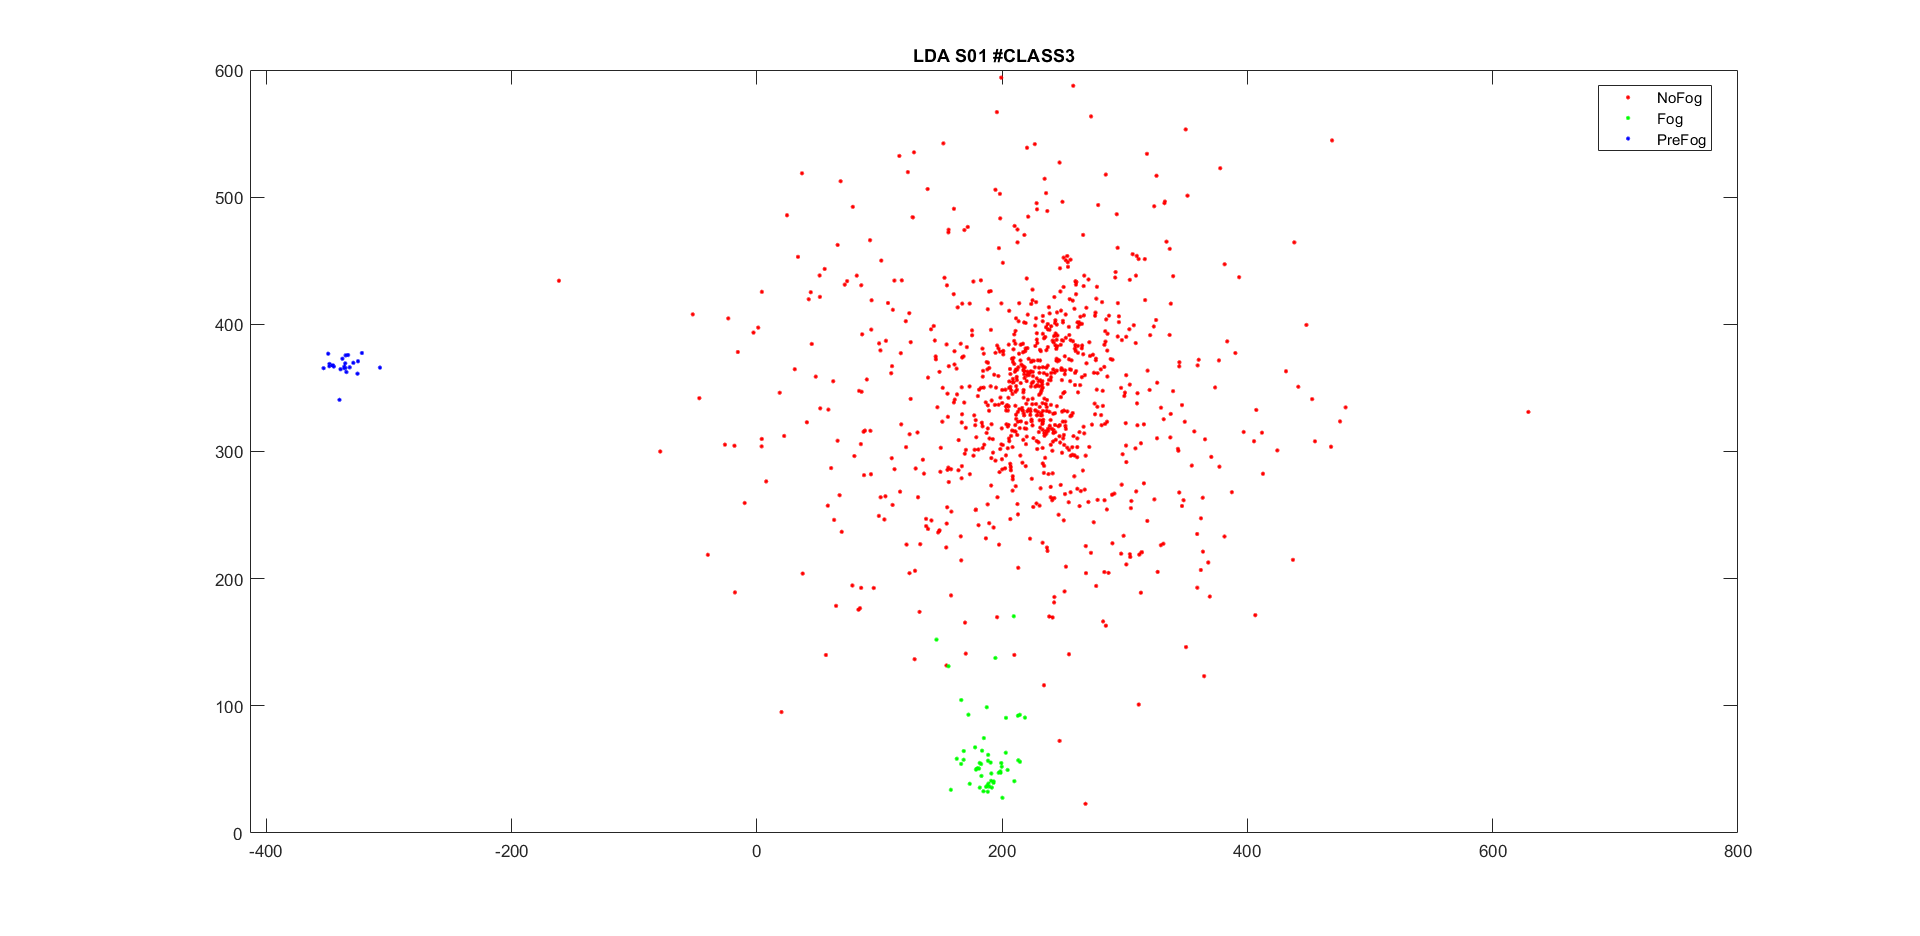
\includegraphics[scale=0.25]{images/LDAS01.png}
	\caption{Grafico delle 3 classi in base alla discriminazione dell'approccio di Fisher per il paziente 1}
	\label{LDAS01}
\end{figure}
\begin{figure}[]
	\centering
	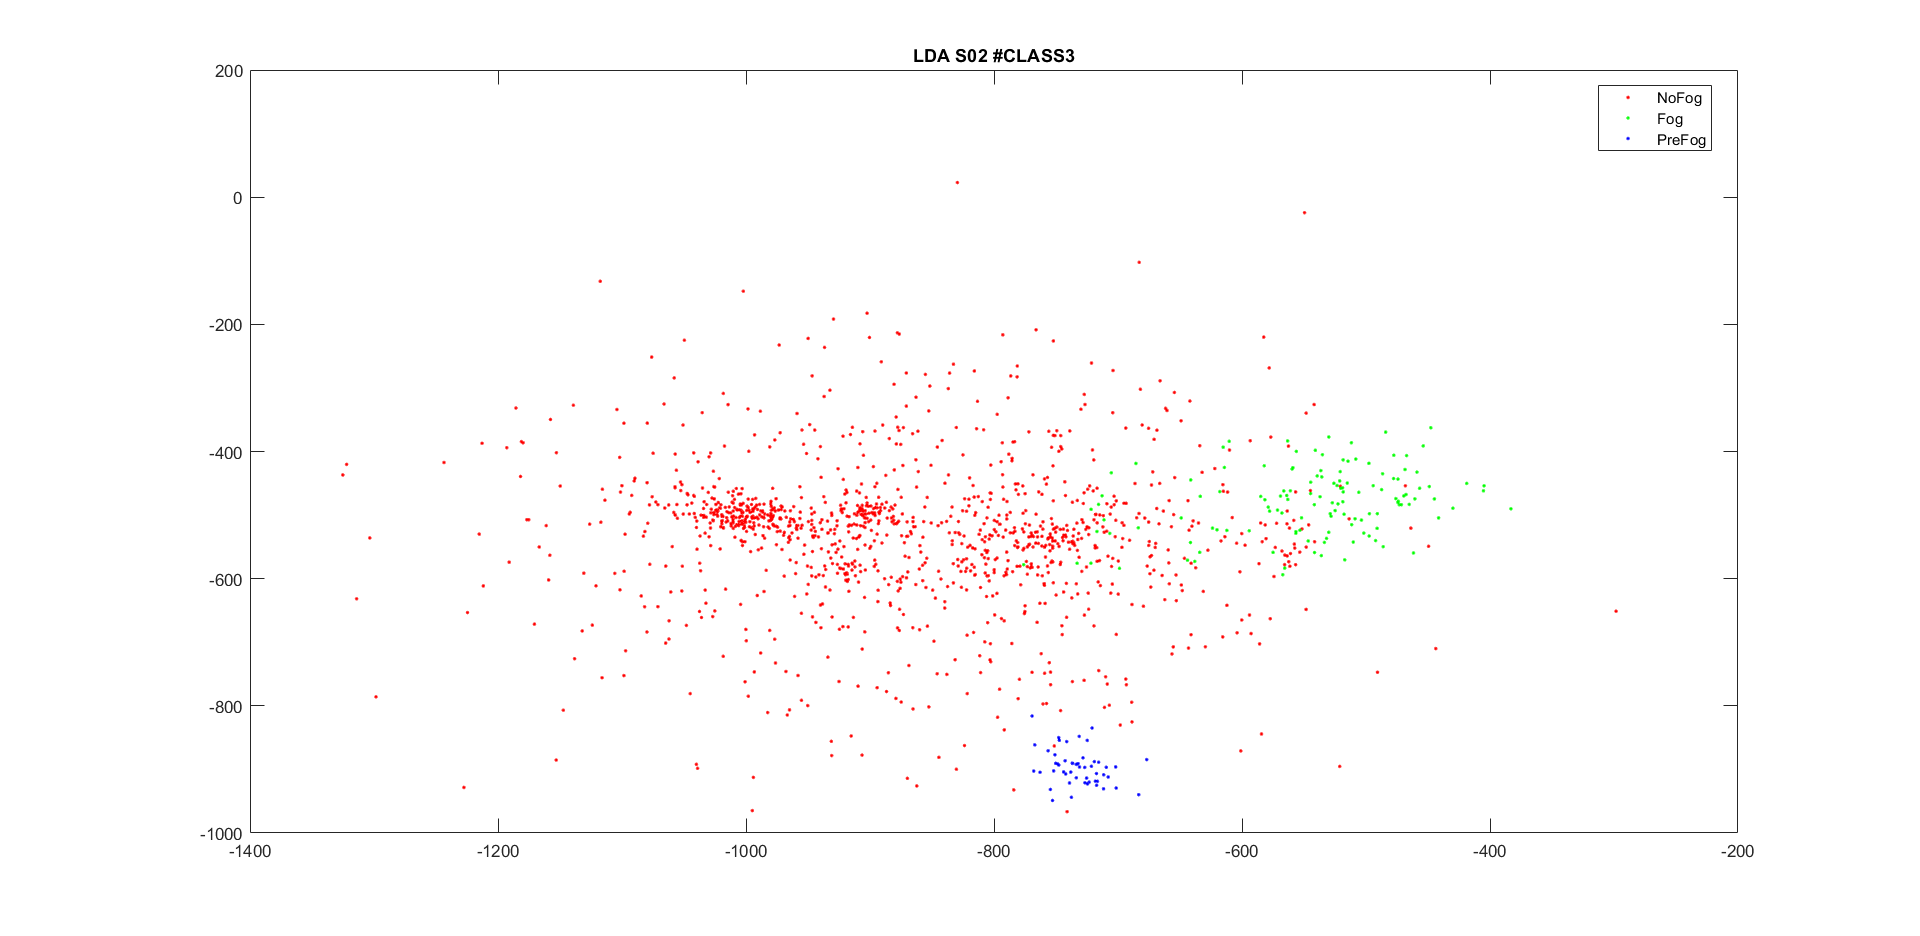
\includegraphics[scale=0.25]{images/LDAS02.png}
	\caption{Grafico delle 3 classi in base alla discriminazione dell'approccio di Fisher per il paziente 2}
	\label{LDAS02}
\end{figure}
\begin{figure}[]
	\centering
	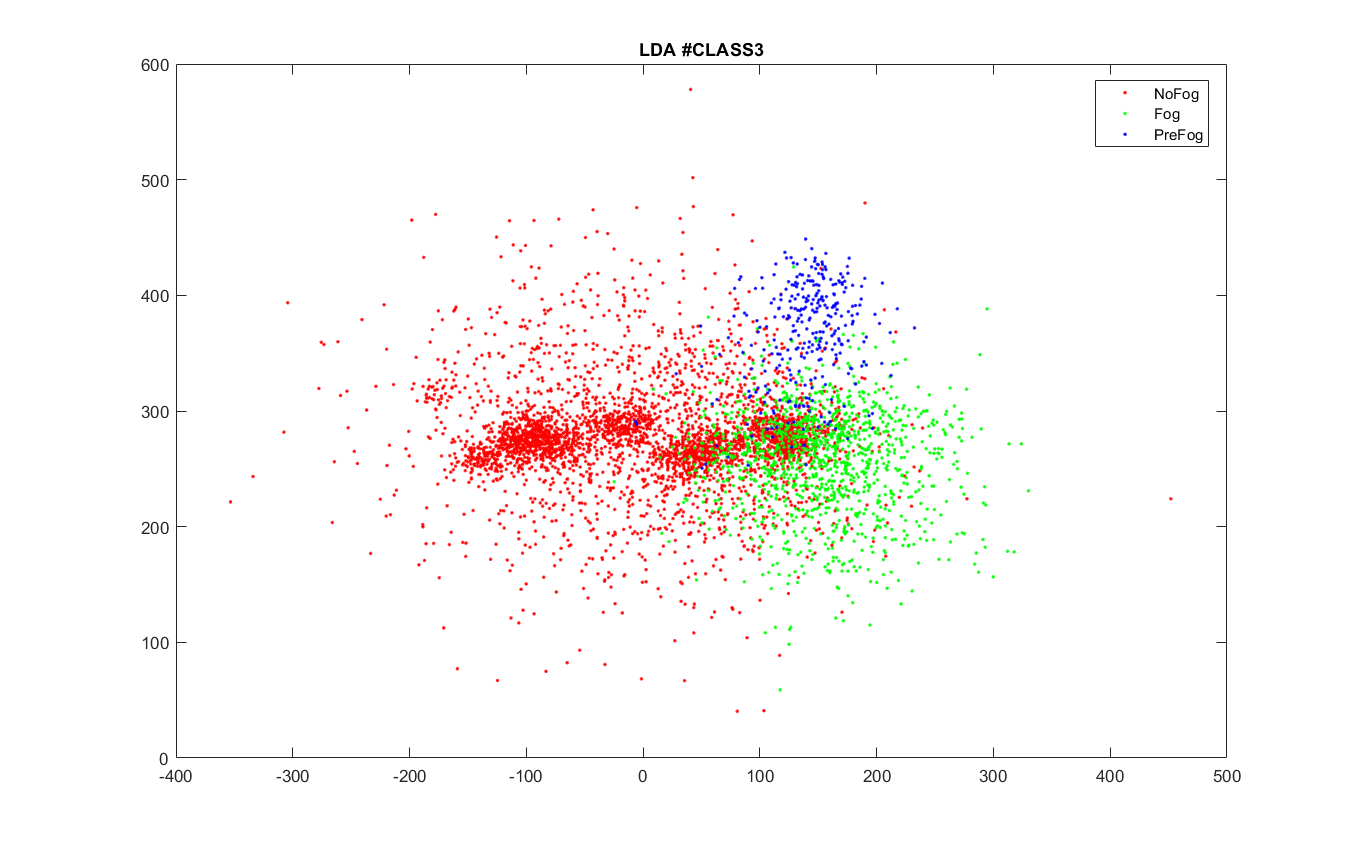
\includegraphics[scale=0.3]{images/LDAALL.png}
	\caption{Grafico delle 3 classi in base alla discriminazione dell'approccio di Fisher presi tutti i pazienti}
	\label{LDAALL}
\end{figure}

\section{Risultati Etichettatura dei dati ed intervalli}
La fase 2 si poneva l'obiettivo di sviluppare un approccio non supervisionato al fine di etichettare i dati provenienti da accelerometri per sostituire il medico e di condurre uno studio sulla migliore divisione temporale dei dati. L'applicazione degli algoritmi di clustering fornisce delle tabelle, per ogni pazienti, in cui vengono espressi i valori di accuratezza, precisione, sensitività e F1-measure. Noi siamo interessati all'intervallo migliore, ossia quello che ci fornisce i valori maggiori delle metriche suddette. Per fare questo, analizziamo ogni tabella e, per ogni algoritmo, salviamo l'intervallo ed i valori che presentano le metriche migliori, come nel caso delle tabelle \ref{ratecmeans}, \ref{ratekmeans}, \ref{rateneuralnetwork}. La metrica riportata per il k means é la square euclidean, in quanto é quella che ci ha portato ad i risultati migliori. \\
Ogni tabella descrive:
\begin{itemize}
	\item l'algoritmo di clustering che é stato utilizzato;
	\item il paziente del test;
	\item i valori delle metriche migliori trovate;
	\item la combinazione overlap-secondi in cui risultano tali metriche.
\end{itemize}

% Please add the following required packages to your document preamble:
% \usepackage{graphicx}
\begin{table}[]
	\centering
	\caption{Rate Pazienti per l'algoritmo di clustering C-means}
	\label{ratecmeans}
	\resizebox{\textwidth}{!}{%
		\begin{tabular}{|l|l|l|l|l|l|l|}
			\hline
			\textbf{}         & \multicolumn{6}{c|}{\textbf{CMEANS}}                                                                              \\ \hline
			\textbf{Paziente} & \textbf{Accuratezza} & \textbf{Precisione} & \textbf{Recall} & \textbf{F1} & \textbf{Overlap} & \textbf{Finestra} \\ \hline
			\textbf{S01}      & 0,92                 & 0,31                & 0,33            & 0,32        & 1                & 2                 \\ \hline
			\textbf{S02}      & 0,44                 & 0,46                & 0,63            & 0,53        & 1                & 2                 \\ \hline
			\textbf{S03}      & 0,7                  & 0,51                & 0,57            & 0,54        & 1                & 2                 \\ \hline
			\textbf{S04}      & 0,7                  & 0,33                & 0               & 0           & 0,5                & 1               \\ \hline
			\textbf{S05}      & 0,53                 & 0,49                & 0,46            & 0,47        & 1                & 1,5               \\ \hline
			\textbf{S06}      & 0,57                 & 0,36                & 0,32            & 0,34        & 1                & 1,5               \\ \hline
			\textbf{S07}      & 0,48                 & 0,37                & 0,43            & 0,4         & 1                & 1,5               \\ \hline
			\textbf{S08}      & 0,41                 & 0,39                & 0,43            & 0,41        & 1,5              & 2                 \\ \hline
			\textbf{S09}      & 0,59                 & 0,35                & 0,37            & 0,36        & 1                & 1,5               \\ \hline
			\textbf{S10}      & 0,73                 & 0,33                & 0               & 0           & 0,5                & 1               \\ \hline
		\end{tabular}%
	}
\end{table}
% Please add the following required packages to your document preamble:
% \usepackage{graphicx}
\begin{table}[]
	\centering
	\caption{Rate Pazienti per l'algoritmo di clustering K-means}
	\label{ratekmeans}
	\resizebox{\textwidth}{!}{%
		\begin{tabular}{|l|l|l|l|l|l|l|}
			\hline
			\textbf{Tutti}    & \multicolumn{6}{c|}{\textbf{KMEANS}}                                                                              \\ \hline
			\textbf{Paziente} & \textbf{Accuratezza} & \textbf{Precisione} & \textbf{Recall} & \textbf{F1} & \textbf{Overlap} & \textbf{Finestra} \\ \hline
			\textbf{S01}      & 0,92                 & 0,72                & 0,34            & 0,46        & 1,5              & 2                 \\ \hline
			\textbf{S02}      & 0,82                 & 0,61                & 0,34            & 0,44        & 1                & 2                 \\ \hline
			\textbf{S03}      & 0,75                 & 0,78                & 0,54            & 0,64        & 1,5              & 2                 \\ \hline
			\textbf{S04}      & 1                    & 0,33                & 0               & 0           & 0,5                & 1               \\ \hline
			\textbf{S05}      & 0,67                 & 0,56                & 0,33            & 0,42        & 1                & 2                 \\ \hline
			\textbf{S06}      & 0,91                 & 0,3                 & 0,33            & 0,32        & 1                & 1,5               \\ \hline
			\textbf{S07}      & 0,92                 & 0,31                & 0,33            & 0,32        & 1                & 2                 \\ \hline
			\textbf{S08}      & 0,7                  & 0,57                & 0,34            & 0,42        & 1                & 1,5               \\ \hline
			\textbf{S09}      & 0,81                 & 0,6                 & 0,34            & 0,43        & 1                & 2                 \\ \hline
			\textbf{S10}      & 1                    & 0,33                & 0               & 0           & 0,5                & 1,5               \\ \hline
		\end{tabular}%
	}
\end{table}
% Please add the following required packages to your document preamble:
% \usepackage{graphicx}
\begin{table}[]
	\centering
	\caption{Rate Pazienti per l'algoritmo di clustering Self-Organizing Map}
	\label{rateneuralnetwork}
	\resizebox{\textwidth}{!}{%
		\begin{tabular}{|l|l|l|l|l|l|l|}
			\hline
			\textbf{Tutti}    & \multicolumn{6}{c|}{\textbf{NEURAL NETWORK}}                                                                      \\ \hline
			\textbf{Paziente} & \textbf{Accuratezza} & \textbf{Precisione} & \textbf{Recall} & \textbf{F1} & \textbf{Overlap} & \textbf{Finestra} \\ \hline
			\textbf{S01}      & 0,92                 & 0,31                & 0,33            & 0,32        & 1                & 1,5               \\ \hline
			\textbf{S02}      & 0,81                 & 0,44                & 0,34            & 0,38        & 1                & 1,5               \\ \hline
			\textbf{S03}      & 0,75                 & 0,78                & 0,54            & 0,63        & 1                & 2                 \\ \hline
			\textbf{S04}      & 0,64                 & 0,33                & 0               & 0           & 0,5                & 1                 \\ \hline
			\textbf{S05}      & 0,58                 & 0,42                & 0,46            & 0,44        & 1                & 2                 \\ \hline
			\textbf{S06}      & 0,57                 & 0,32                & 0,31            & 0,31        & 1                & 1,5               \\ \hline
			\textbf{S07}      & 0,63                 & 0,3                 & 0,26            & 0,28        & 1                & 2                 \\ \hline
			\textbf{S08}      & 0,56                 & 0,69                & 0,38            & 0,49        & 1,5              & 2                 \\ \hline
			\textbf{S09}      & 0,57                 & 0,37                & 0,41            & 0,39        & 1                & 2                 \\ \hline
			\textbf{S10}      & 1                    & 0,33                & 0               & 0           & 0,5                & 1               \\ \hline
		\end{tabular}%
	}
\end{table}
Dalle tabelle, si nota come il valore di overlap e dimensione della finestra che più frequentemente mi portano ad avere metriche migliori sono:
\begin{itemize}
	\item 1 secondo di sovrapposizione e 2 secondi di finestra;
	\item 1 secondo di sovrapposizione e 1,5 secondi di finestra.
\end{itemize}
L'obiettivo di sostituire il medico nella prima fase di test, ossia raccogliere dati dagli accelerometri ed applicare le etichette di noFOG, FoG o preFOG, sembra fattibile, in quanto in molti casi abbiamo un'accuratezza vicina al 90\% o comunque superiore al 70\%, per cui la maggior parte delle volte il clustering segna l'etichetta come corretta. Un fatto interessante da notare è che nel caso di pazienti che non hanno avuto episodi di FoG, come il 4 ed il 10, l'accuratezza sia del 100\%, suggerendoci che i movimenti di camminata normale siano comunque diversi da quelli di FoG o preFOG e quindi vengono riconosciuti come tutti simili in assenza di Freezing.\\
\subsection{LDA con intervallo migliore}
In \ref{LDAS01} e \ref{LDAS02} si era notato come esiste una certa distinzione tra le classi, ma restava una sovrapposizione tra alcuni dati di esse, il che ci porta a studiare quale sia il miglior intervallo di divisione dei dati. Analogamente al procedimento per la fase di clustering, iteriamo l'algoritmo di LDA cambiando la durata della finestra temporale e la sovrapposizione tra di essi. Gli intervalli possibili, come nel caso del clustering, vanno da 1 a 5 secondi per la finestra, da 0.5 a 4.5 secondi per la sovrapposizione.\\
Dopo aver provato tutte le possibili combinazioni, risulta anche in questo caso che scegliendo 2 secondi di finestra ed 1 secondo di overlap si ottiene una divisione molto più netta per il singolo paziente, come si può vedere in \ref{LDAS01_best.png} e \ref{LDAS02_best.png}.\\
Anche usando i dati di tutti i pazienti si può notare, in figura \ref{LDAALL2.png}, che c'è un miglioramento nella divisione dei dati, soprattutto considerando il preFOG, usando un intervallo di 2 secondi per la finestra ed 1 secondo per l'overlap.
\begin{figure}[]
	\centering
	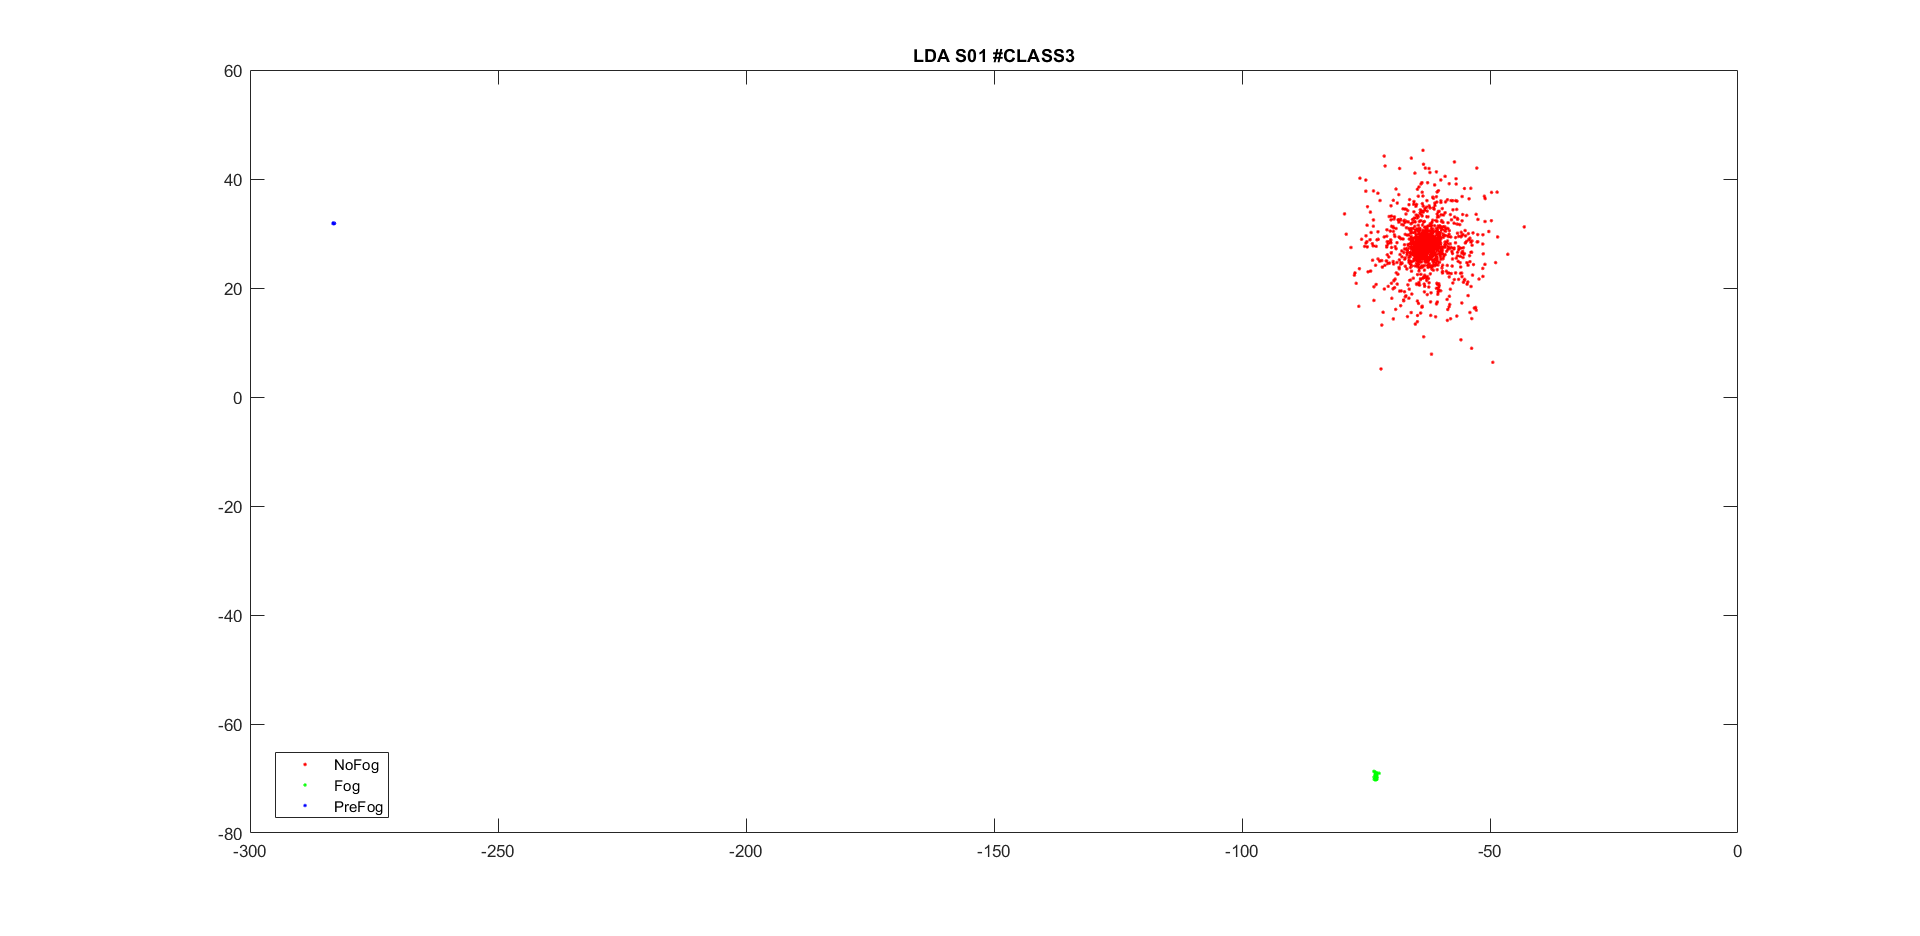
\includegraphics[scale=0.25]{images/LDAS01_best.png}
	\caption{Grafico delle 3 classi in base alla discriminazione dell'approccio di Fisher per il paziente 1 con 2 secondi di finestra ed 1 secondo di overlap}
	\label{LDAS01_best.png}
\end{figure}
\begin{figure}[]
	\centering
	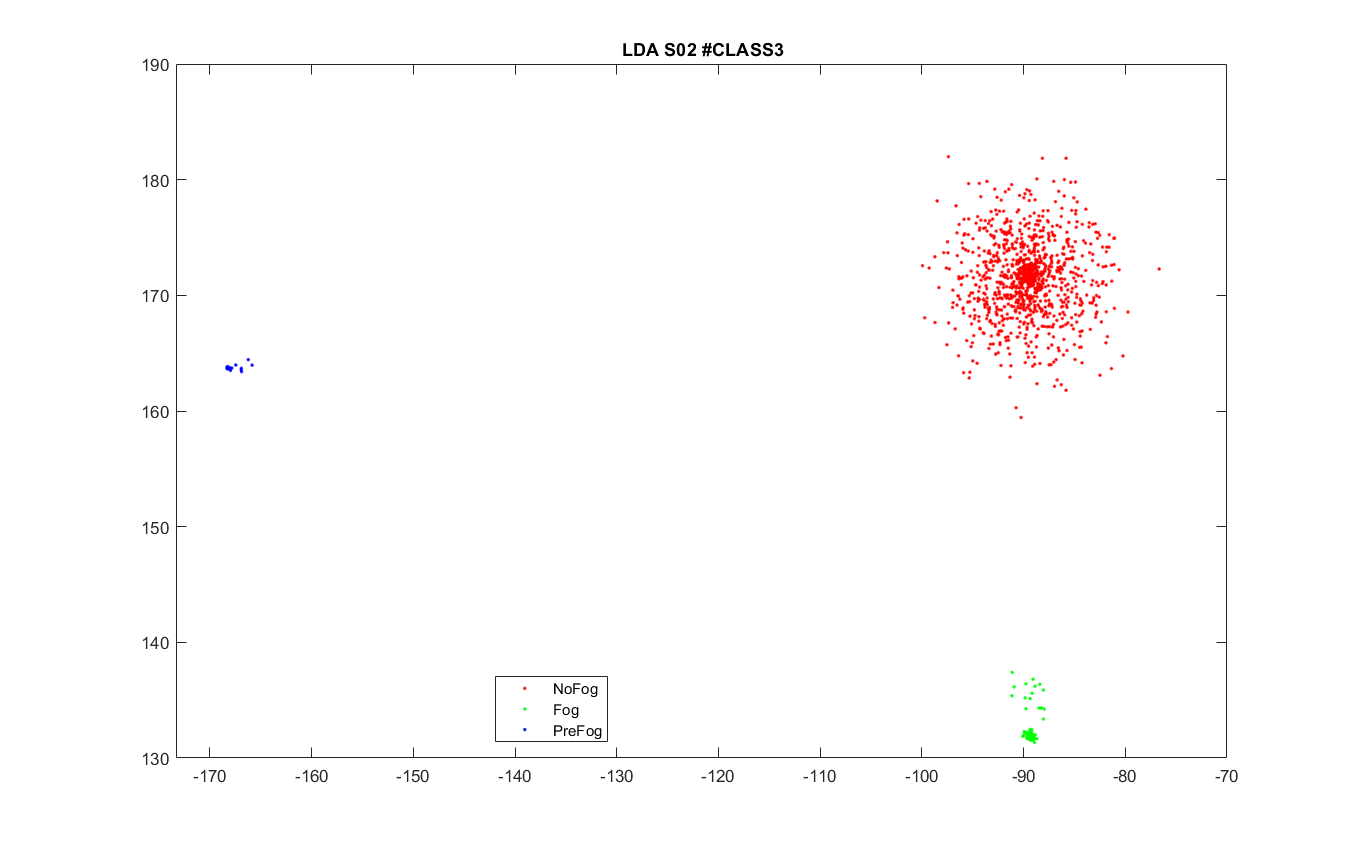
\includegraphics[scale=0.3]{images/LDAS02_best.png}
	\caption{Grafico delle 3 classi in base alla discriminazione dell'approccio di Fisher per il paziente 2 con 2 secondi di finestra ed 1 secondo di overlap}
	\label{LDAS02_best.png}
\end{figure}
\begin{figure}[]
	\centering
	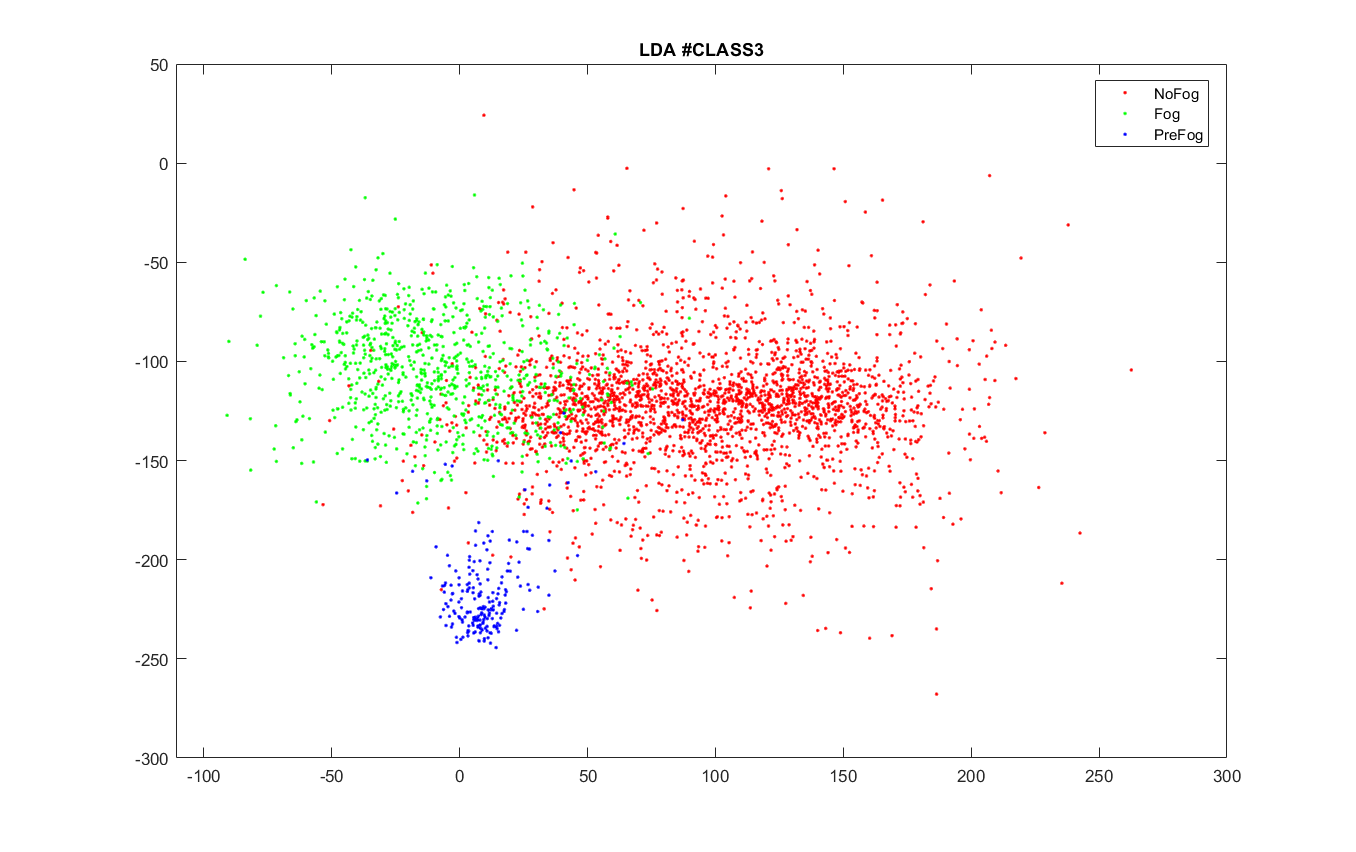
\includegraphics[scale=0.3]{images/LDAALL2.png}
	\caption{Grafico delle 3 classi in base alla discriminazione dell'approccio di Fisher per tutti i pazienti con 2 secondi di finestra ed 1 secondo di overlap}
	\label{LDAALL2.png}
\end{figure}
Il nostro studio degli intervalli, sia per la parte non supervisionata che per la parte di LDA, ci porta a concludere che il miglior modo con cui si possono dividere i dati in finestre per calcolare le feature é quello di scegliere 1 secondo per la sovrapposizione tra le finestre ed 1,5 o 2 secondi per quanto riguarda la lunghezza della finestra temporale.

\section{Risultati Classificazione}
\subsection{Risultati sul singolo paziente}
Per ogni paziente su cui è stata effettuata la prova, abbiamo ricavato la media delle matrici di confusione della cross-validation. Successivamente, prendendo un altro dataset dello stesso paziente, utilizzando il knn allenato abbiamo cercato di predire le classi del secondo dataset. Poiché non tutti i pazienti presentano, nel dataset, due diversi file (ossia due prove di camminata), la prova è stata possibile solo su alcuni di essi.\\
In tabella \ref{MCcross1} possiamo osservare le matrici di confusione della cross-validation a 10 gruppi per i pazienti numero 1, 2, 3, 5, 7, ossia quelli con doppio file. Si può notare come la matrice risulti diagonali, il che vuole dire che etichetta, nella cross-validation, sempre giusti i nostri campioni sullo stesso paziente.\\
In tabella \ref{MCprev1}, ossia quella relativa alla predizione su un nuovo file, osserviamo che la matrice è abbastanza più confusa, per cui alcune volte etichetta occorrenze di preFOG come altro e non casi di preFOG come preFOG. In tabella \ref{Mpred} si possono osservare le metriche di accuratezza, sensitività, specificità ed F1-measure per la predizione.\\
Questo risultato può essere dato dal fatto che, anche per lo stesso paziente, percorsi diversi o situazioni diverse portano ad una camminata differente da quelle precedenti, e quindi ho dati che possono risultare molto simili ma appartenere a casi diversi nei due test. La cross-validation restituisce delle metriche perfette, quindi l'algoritmo riesce a classificare molto bene i punti di un dataset anche allenandosi solo su una parte di esso e prevedendo i dati esclusi.\\
Il caso della previsione su dati di file diversi, invece, è  da migliorare, in quanto restituisce una specificità bassa, ossia tende a confondere preFOG in NoFoG o FoG. Questo fatto può essere dovuto al fatto che i movimenti, e quindi i dati, di preFOG sono altamente soggettivi e dipendenti dalla situazione in cui il paziente si trova, quindi un movimento nuovo può essere classificato male rispetto al dataset di training. Una possibile soluzione a questo problema sarebbe quello di ottenere dei dataset più grandi, in modo tale da avere un maggior numero di movimenti su cui allenare il classificatore.
% Please add the following required packages to your document preamble:
% \usepackage{multirow}
% \usepackage{graphicx}
\begin{table}[]
	\centering
	\caption{Matrici di confusione per la cross-validation del singolo paziente}
	\label{MCcross1}
	\resizebox{\textwidth}{!}{%
		\begin{tabular}{|c|l|c|c|c|c|c|c|c|c|c|c|}
			\hline
			\textbf{Paziente}                                                                       &                & \textbf{01}                       & \textbf{}                        & \multicolumn{2}{c|}{\textbf{02}}                                     & \multicolumn{2}{c|}{\textbf{03}}                                     & \multicolumn{2}{c|}{\textbf{05}}                                     & \multicolumn{2}{c|}{\textbf{07}}                                     \\ \hline
			\multicolumn{1}{|l|}{}                                                                  & \textbf{Label} & \multicolumn{1}{l|}{\textbf{NPF}} & \multicolumn{1}{l|}{\textbf{PF}} & \multicolumn{1}{l|}{\textbf{NPF}} & \multicolumn{1}{l|}{\textbf{PF}} & \multicolumn{1}{l|}{\textbf{NPF}} & \multicolumn{1}{l|}{\textbf{PF}} & \multicolumn{1}{l|}{\textbf{NPF}} & \multicolumn{1}{l|}{\textbf{PF}} & \multicolumn{1}{l|}{\textbf{NPF}} & \multicolumn{1}{l|}{\textbf{PF}} \\ \hline
			\multirow{2}{*}{\textbf{\begin{tabular}[c]{@{}c@{}}Matrice \\ Confusione\end{tabular}}} & \textbf{NPF}   & 1413                              & 0                                & 431                               & 0                                & 1335                              & 0                                & 983                               & 0                                & 1127                              & 0                                \\ \cline{2-12} 
			& \textbf{PF}    & 0                                 & 36                               & 0                                 & 18                               & 0                                 & 84                               & 0                                 & 76                               & 0                                 & 32                               \\ \hline
		\end{tabular}%
	}
\end{table}
% Please add the following required packages to your document preamble:
% \usepackage{multirow}
% \usepackage{graphicx}
\begin{table}[]
	\centering
	\caption{Matrici di confusione per la previsione del singolo paziente}
	\label{MCprev1}
	\resizebox{\textwidth}{!}{%
		\begin{tabular}{|c|l|c|c|c|c|c|c|c|c|c|c|}
			\hline
			\textbf{Paziente}                                                                       &                & \textbf{01}                       & \textbf{}                        & \multicolumn{2}{c|}{\textbf{02}}                                     & \multicolumn{2}{c|}{\textbf{03}}                                     & \multicolumn{2}{c|}{\textbf{05}}                                     & \multicolumn{2}{c|}{\textbf{07}}                                     \\ \hline
			\multicolumn{1}{|l|}{}                                                                  & \textbf{Label} & \multicolumn{1}{l|}{\textbf{NPF}} & \multicolumn{1}{l|}{\textbf{PF}} & \multicolumn{1}{l|}{\textbf{NPF}} & \multicolumn{1}{l|}{\textbf{PF}} & \multicolumn{1}{l|}{\textbf{NPF}} & \multicolumn{1}{l|}{\textbf{PF}} & \multicolumn{1}{l|}{\textbf{NPF}} & \multicolumn{1}{l|}{\textbf{PF}} & \multicolumn{1}{l|}{\textbf{NPF}} & \multicolumn{1}{l|}{\textbf{PF}} \\ \hline
			\multirow{2}{*}{\textbf{\begin{tabular}[c]{@{}c@{}}Matrice \\ Confusione\end{tabular}}} & \textbf{NPF}   & 412                               & 27                               & 808                               & 173                              & 229                               & 20                               & 621                               & 354                              & 343                               & 90                               \\ \cline{2-12} 
			& \textbf{PF}    & 9                                 & 1                                & 23                                & 10                               & 9                                 & 1                                & 40                                & 14                               & 11                                & 5                                \\ \hline
		\end{tabular}%
	}
\end{table}

% Please add the following required packages to your document preamble:
% \usepackage{graphicx}
\begin{table}[]
	\centering
	\caption{Metriche di misura della predizione per il singolo paziente}
	\label{Mpred}
	\resizebox{\textwidth}{!}{%
		\begin{tabular}{|c|c|c|c|c|}
			\hline
			\multicolumn{1}{|l|}{\textbf{Paziente}} & \multicolumn{1}{l|}{\textbf{accuratezza}} & \multicolumn{1}{l|}{\textbf{sensitività}} & \multicolumn{1}{l|}{\textbf{specificità}} & \multicolumn{1}{l|}{\textbf{F1-measure}} \\ \hline
			\textbf{S01}                            & 0.9198                                 & 0.9385                                    & 0.1000                                    & 0.9581                                   \\ \hline
			\textbf{S02}                            & 0.8067                                 & 0.8236                                    & 0.3030                                    & 0.8918                                   \\ \hline
			\textbf{S03}                            & 0.8880                                 & 0.9197                                    & 0.1000                                    & 0.9404                                   \\ \hline
			\textbf{S05}                            & 0.6171                                 & 0.6369                                    & 0.2593                                    & 0.7591                                   \\ \hline
			\textbf{S07}                            & 0.7751                                 & 0.7921                                    & 0.3125                                    & 0.8716                                   \\ \hline
		\end{tabular}%
	}
\end{table}

\subsection{Risultati usando i dati di tutti i pazienti}
Andando ad usare i dati provenienti da tutti i pazienti, si può osservare in tabella \ref{MCall}, che rappresenta la media delle matrici di confusione della cross-validation e le metriche di accuratezza, sensitività, specificità e F1-measure, come la matrice di confusione non sia diagonale come nel caso del paziente singolo, in quanto pazienti diversi hanno modi di camminare differenti e quindi porta ad avere dati diversi, i quali possono essere classificati nel modo sbagliato. Le metriche comunque sono molto buone, il che ci porta a supporre che molti movimenti di preFOG sono comuni e quindi si può procedere con un modello futuro di previsione di nuovi dati, magari avendo a disposizione dei dataset più grandi ed un numero maggiore di pazienti.
\begin{table}[]
	\centering
	\caption{Matrice confusione e metriche di misura della cross-validation con i dati di tutti i pazienti}
	\label{MCall}
	\resizebox{\textwidth}{!}{%
		\begin{tabular}{|c|l|c|c|c|c|c|c|}
			\hline
			\multicolumn{1}{|l|}{}                                                                  & \textbf{Label} & \multicolumn{1}{l|}{\textbf{NPF}} & \multicolumn{1}{l|}{\textbf{PF}} & \multicolumn{1}{l|}{\textbf{accuratezza}} & \multicolumn{1}{l|}{\textbf{sensitività}} & \multicolumn{1}{l|}{\textbf{specificità}} & \multicolumn{1}{l|}{\textbf{F1-measure}} \\ \hline
			\multirow{2}{*}{\textbf{\begin{tabular}[c]{@{}c@{}}Matrice \\ Confusione\end{tabular}}} & \textbf{NPF}   & 8426                              & 898                              & 0.90                                   & 0.90                                    & 0.89                                 & 0.95                                     \\ \cline{2-8} 
			& \textbf{PF}    & 39                                & 309                              &                                        &                                         &                                      &                                          \\ \hline
		\end{tabular}%
	}
\end{table}
